The phase-by-phase (PP) system was developed to overcome a number of deficiencies, which seemed widespread in adaptive systems:

\begin{itemize}
\item Fixed cycle length and/or fixed step for variation of cycle length
\item Utilization of aggregated demand data only
\item Fixed coordination of signals along an arterial og through a network
\end{itemize}

The proposed overall scheme to improve upon these issues are the isolated optimization of intersections and more fine-grained tracking of vehicles.

The optimization process has been made independent from determination of the network state ie. detection and prediction and as such some of these subjects are mostly discussions and proposals for improvements.

\subsubsection*{Detection}
PP relies on individual tracking of vehicles to obtain an arrival based model. For networks this can be realized only with video detection with eg. license plate recognition; traditional loop detections cannot yet identify individual vehicles.

The PP system currently works for isolated intersections and so detection loops are sufficient to estimate arrival times. For detector placement, the authors suggest using simulation.

\subsubsection*{Prediction}
In the proposed form the PP system uses a Poisson process to generate interarrival times.
Alternatives are some form of time-series analysis or a Poisson process with variable mean. The use of detections made upstream could also be used, such as it is in RHODES.

The performance of PP is highly dependent on the ability of the chosen prediction system to generate proper forecasts but, as will be seen in the test results, the potential benefits are great.

\subsubsection*{Optimization}
The optimization procedure of PP seeks to minimize the stopped delay using input from the prediction process. The most widely used measure of effectiveness is stopped delay (see eg. \cite{9}, \cite{38} and \cite{31}) but the authors show that there is also a linear relationship to total travel time.

The following notation is used in the paper:

\begin{table}[!ht]
\begin{center}
\begin{tabular}{ll}
\hline
$H$ & Horizon of optimization \\
$cs$ & Cycle start time \\
$ce = cs+H$ & Cycle end time \\
$i = 1,...,N$ & Approach indexes \\
$k = 1,...,M$ & Phase indexes \\
$\lambda_k$ &  Is a partitioning of $H$ into phases and $0 = \lambda_{0} <  \lambda_{k-1} \leq \lambda_k \leq 1$ \\
$\lambda_{k_i}$ & The time into $H$ before the phase $k$, involving approach $i$, ends \\
$j$ & Vehicle id for predicted vehicle arrival within the horizon  \\
$t_{ij}$ & The arrival time for vehicle $j$ on approach $i$
\\ \hline
\end{tabular}
\end{center}
\caption{Notation}
\end{table}

$H$ should be in the order of the desired cycle time and $\lambda_k$ give the green splits and thus we have a full plan for the signal. Stopped delay can be calculated from this plan and the predicted arrivals. In Figure \ref{fig:pp_delay} this idea is sketched.

\begin{figure}[!ht]
\begin{center}
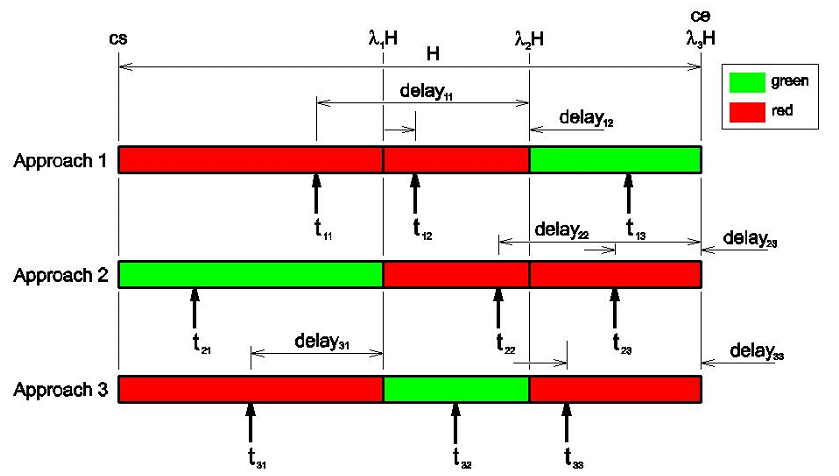
\includegraphics[scale=0.5]{phase-by-phase_delay-model.png} 
\end{center}
\caption{Calculation of stopped delay in the Phase-by-Phase system for an intersection with 3 approaches and 1 exit (no turning movements).}
\label{fig:pp_delay}
\end{figure}

In equation \ref{eqn:pp_delay} the rules for stopped delay are extracted when vehicle $j$ arrives on approach $i$ at $t_{ij}$.

\begin{equation}
delay = 
\begin{cases}
cs + H \cdot \lambda_{k_i-1} - t_{ij} & when \; t_{ij} \leq cs + H \cdot \lambda_{k_i-1} \; (before\;green)  \\
cs + H - t_{ij} & when \; t_{ij} \geq cs + H \cdot \lambda_{k_i} \; (after\;green)  \\
0 & otherwise
\end{cases}
\label{eqn:pp_delay}
\end{equation}

In the second case of equation \ref{eqn:pp_delay} vehicles incur stopped delay since they arrive after their approach has been served green time in the planning horizon. Thus they will not be served before the next green, which has not yet been planned, and stopped delay is accumulated until then. This is called carryover since vehicles are carried over into the next cycle.

PP also takes into account queue startup delay and thus cover the most critical sources of delay. However PP makes the assumption that the granting of green time to a phase will cause the approaches to be cleared completely ie. no vehicles must experience more than one green phase before they can leave.

The objective function is defined using these delay terms and thus optimization can be done by making changes in the $\lambda_k$-values within some critical points in horizon. Looking at Figure \ref{fig:pp_delay} it is seen that approach 2 is served green time until $\lambda_1 H$, supressing green from approach 1 and 3, which both have arrivals. By switching phase immediately after $t_{21}$ (setting $\lambda_1 = (t_{21} - cs)/H$) approach 1 could receive green until immediately after $t_{12}$ and so on. This example involves switching of the phase order, which was not considered in the paper.

In the PP paper \cite{1} a solution method using the above scheme is presented as a combinatorial problem. But the number of combinations increase exponentially with the number of arrivals and the number of phases. Therefore a tabu search is employed. Websters formula for optimum green time splits is used in the Proportional Heuristic to obtain a good initial solution and a 1-bit neighborhood function is defined by making changes to a single value in $\lambda_k$ (a low influence move), preserving the phase order. Candidates for the step of these changes range from the transmission time of an electronic signal ($\approx 10^{-3}s$) to the minimum headway between two vehicles travelling in a platoon ($\approx 2s$ cf. Greenshields et al. 1947).
A high influence move, which reorders phases, is also described but is not included, as mentioned.

\subsubsection*{Evaluation}
Shenoda and Machemel compares the results of their metaheuristic search to pretimed and actuated signal control settings obtained from the CORSIM microsimulator using the test intersection in Figure \ref{fig:pp_intersection}.

\begin{figure}[!ht]
\begin{center}
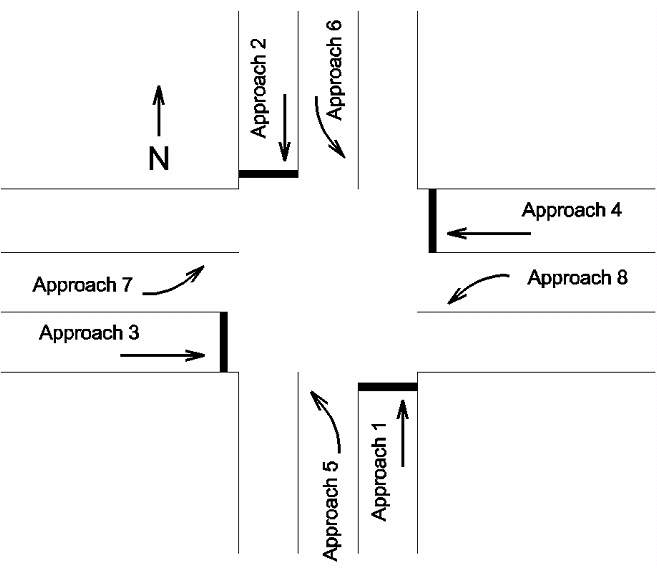
\includegraphics[scale=0.5]{phase-by-phase_testing-intersection.png} 
\end{center}
\caption{4-phase intersection from experiment \#2}
\label{fig:pp_intersection}
\end{figure}

The intersection was subjected to 8 different data sets of arrival times. In Figure \ref{fig:pp_improvements} the stopped delays for the PP system is compared to the simulation results using pretimed plans and standard traffic actuated control.

\begin{figure}[!ht]
\begin{center}
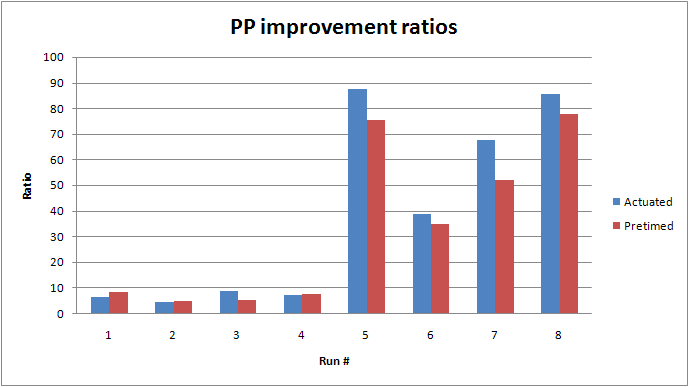
\includegraphics[scale=0.5]{phase-by-phase_improvement_ratios.png} 
\end{center}
\caption{Improvement factors of PP compared to pretimed and actuated control in the 4-phase intersection of Figure \ref{fig:pp_intersection}}
\label{fig:pp_improvements}
\end{figure}

The results should only be taken as indications since a number of assumptions were made for PP that the prediction algorithm supplied perfect information. In addition the actuated control was only semi-actuated since detectors were only used in one direction, the other being timed as in the pretimed case, which was optimized using Websters formulas.

In spite of these issues it is interesting to observe that the (semi-)actuated control strategy is not always superior to pretimed plans. It is clear, however, that both strategies are outperformed by PP. Under the given assumptions - in particular that concerning accuracy of predictions - PP can be used to establish a baseline for the best possible performance. This becomes even more true when the phase ordering constraint is dropped allowing reordering and skipping of phases.

Unfortunately Shenoda and Machemehl do not test PP on a network or even along an arterial. The optimization procedure does not consider coordination in itself though it is proposed that the prediction routine should consider departures from adjacent intersections, such as the method by Head employed in RHODES. It is speculated that such propagation of departure information could give rise to some coordination, depending on the horizon of optimization.